\section{Lesson 5, 07/10}
These non-physical isothermals appear under a critical temperature $T_c$, determined
by the parameters $a,b$.

[equation of correspondent states]
\subsection{Coexistence of many phases}
Consider a $p,V,T$ system with 1 type of component: at most three phases can coexist,
because the equality of the chemical potentials depends only on 2 variables $p,T$, so
only 2 conditions can have a single solution
$$\begin{dcases*}
\mu_\alpha(p,T) = \mu_\beta(p,T)\\
\mu_\beta(p,T) = \mu_\gamma(p,T)
\end{dcases*}.
$$
The 3 phases can coexist at most in single points, called \textit{triple points}.

\textbf{Example: triple point of water}
\begin{figure}[H]
    \centering
    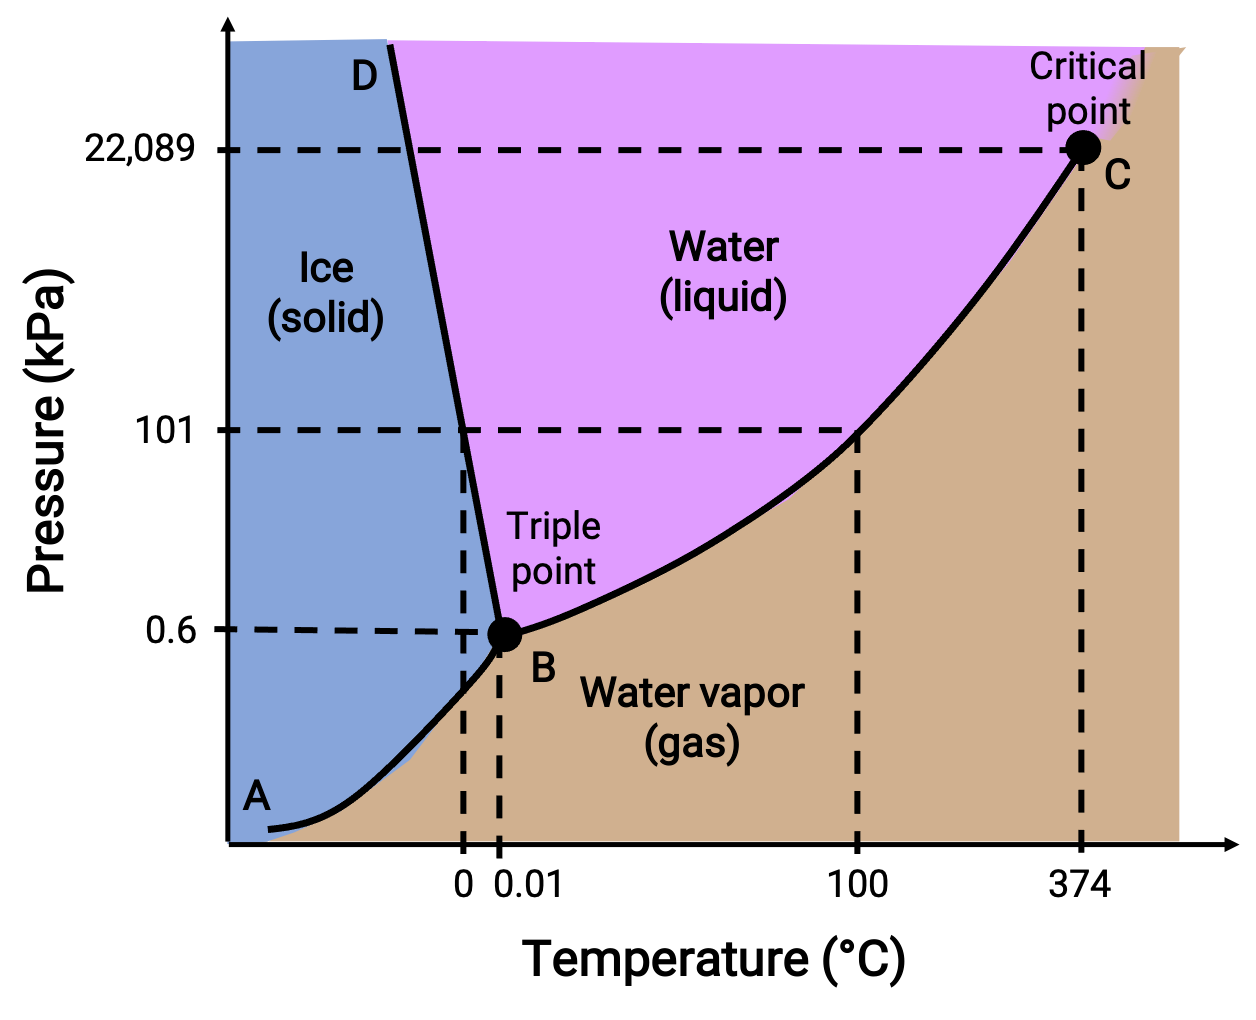
\includegraphics[width = .5\linewidth]{./triple_water.png}
    \caption{\small The phase diagram of water.}
\end{figure}
The liquid-gas transition is continuous, but the coexistence line has an end, this
means that their distinction is well-defined only "close" to the first order
transition and that they are not so different from each other (they share the same
symmetry in structure); at the critical point there usually is a partial symmetry
breaking.
\subsection{Gibbs rule}
This is a statement about the number of phases that can coexist in multi-component
systems.\\
Consider a system with $c$ components (indexed by $i=1,2..c$), which presents $f$
phases at equilibrium (indexed by $\alpha = 1,2...f$); the portion of particles of
type $i$ in phase $\alpha$ is denoted by $\nu_{i,\alpha}$. For all $\alpha$,
it is true that
$$\sum_{i=1}^{c}\nu_{i,\alpha} = 1 $$
so these are $f\cdot(c-1)$ constraints.\\
Moreover, for every component $i$ the chemical potentials for each phase must be
the same
$$\mu_{i,1}(T,p,\nu_{1,1},...\nu_{c-1,1})=\mu_{i,2}(...) = \mu_{i,3}=...=\mu_{i,f}$$
these are $f-1$ independent equations for every $i$, so these are $c(f-1)$
constraints.

So in total, the independent variables are
$2+c-f$ and
this number must be positive, so the Gibbs rule states that
$$2+c-f\geq0$$\\

\chapter{Statistical Mechanics}
\subsection{Statistical approach to TD}
Thermodynamic systems contain very large numbers of particles, $N\sim\mathcal{N}_A\sim
10^{23}$, so the possible states are characterized by a large number of quantum
numbers/canonical coordinates ($6N$ for point-like classic particles).\\
\textbf{Example} For quantum harmonic oscillators the microstates can be determined
by the $3$ quantum number for every oscillator, so a generic state is
$$\ket{\nu(t)}=\sum_{A}^{}C_A(t)\ket{\mathbf{n}_1,\mathbf{n}_2,...\mathbf{n}_N}.$$\\

Microstates evolve according to microscopic dynamics: Hamilton's equations
$$\begin{dcases*}
\dot q^A = \pdv{H}{p_A}\\
\dot p_A = -\pdv{H}{q^A}
\end{dcases*}
$$
are $3N$ equations that, along with $6N$ initial conditions, completely determine the
motion of the system.\\
\textbf{Observation}: the classical evolution is at odds with thermodynamics for 2
reasons:
\begin{enumerate}
    \item Hamilton's equations obey the time-reversal symmetry, while the second
        principle of thermodynamics prescribes a preferential direction of the
        evolution of the system;
    \item Poincaré cycles states that, if a phase space is limited, the trajectory
        of the system will return arbitrarily close to the starting point, given
        enough time.\\
\end{enumerate}

This microscopic approach is not only inconceivable, since it involves solving
$\sim\mathcal{N}_A$ coupled PDEs, but also redundant, as in TD the state of a gas
could be determined with only a handful of macroscopic variables. The set of these
variables is called a \textbf{macrostate} and each one includes a huge number of
microstates: this state is at equilibrium, but the system still moves in the phase
space and "visits" many microstates of the macrostate.\\

\subsection{Observables}
To measure an observable, the whole microstate must be known and the observable must
be measured instantaneously: the value of the observable is the mean of the values
found
$$O_\text{obs} = \frac{1}{M}\sum_{n=1}^{M}O_n$$
and the mean value in time is the integral mean over time on the system trajectory 
$\nu(t)$
$$\bar O = \frac{1}{T}\int_{0}^{T}\dd t O(\nu(t)).$$\\

The statistical approach is different, the value is found using the average in terms
of frequencies: given the set of microstates $\left\{\nu\right\}$, the value is
$$O_\text{obs} = \sum_{\left\{\nu\right\}}^{} \frac{n(\nu)}{M}O(\nu)$$
where $n(\nu)$ is the number of times ????

This is similar to the definition of a mean value, with $P(\nu) = \frac{n(\nu)}{M}$:
since the microstates are points in the phase space, the probability should be
expressed in terms of an integral
$$\langle O\rangle = \int_{}^{}\dd\mu \rho(q,p)O(q,p)=\int_{}^{}\dd q\land\dd p
\rho(q,p)O(q,p)$$
where $\rho(q,p)$ is the probability that the microstate falls into an (hyper-)cube
around $(q,p)$; the main objective of statistical mechanics is to determine this
probability density.

In general, for non-equilibrium states, the density evolves with time, but this
evolution is determined by the \textit{Liouville Theorem}.\\
\textbf{Liouville Theorem}\\
If a probability density $\rho(q,p,t)$ satisfies a continuity equation, then
$$\dv[]{\rho}{t} = \pdv[]{\rho}{t} + \sum_{A}^{}\left(\pdv{\rho}{q^A}\dot q_A +
\pdv[]{\rho}{p_A}\dot p_A\right)=\pdv[]{\rho}{t}+\left\{\rho,H\right\}=0$$
\textbf{Proof}\\
The continuity equation is
$$\pdv[]{\rho}{t} + \divergence\mathbf{j}=0$$
and the associated current $\mathbf{j}$ is given by "density times velocity", which
in the phase space is
$$\mathbf{j} = \left(\rho\dot q^A,\rho\dot p_A\right)$$
expanding the divergence
$$0=\pdv[]{\rho}{t} + \pdv{}{q^A}\left(\rho\dot q^A\right)+\pdv{}{p_A} \left(\rho\dot
p_A\right) = \pdv[]{\rho}{t}+ \pdv{\rho}{q^A}\dot q^A + \pdv[]{\rho}{p_A}\dot p_A +
\rho\left(\pdv{\dot q^A}{q^A} + \pdv{\dot p_A}{p_A}\right)$$
recalling Hamilton's equations and commuting second derivatives yields the result.
